\graphicspath{{images/}}

\section{Методы приближения функций}

\subsection{Полиномиальная интерполяция}

\subsubsection{Постановка задачи}
Используя таблицу значений $Y_i$ функции $y = f(x)$, вычисленных в точках $X_i$, $i = 0, \dots ,3$  построить интерполяционные многочлены Лагранжа и Ньютона, проходящие через точки $\{X_i, Y_i\}$. Вычислить значение погрешности интерполяции в точке $X^*$.

\subsubsection{Консоль}
\begin{alltt}
$ make
g++ -g -pedantic -std=c++17 -Wall -Wextra -Werror main.cpp -o solution
$ cat tests/1.in
4
-3 -1 1 3
-0.5
$ ./solution < tests/1.in
Интерполяционный многочлен Лагранжа: 0.831529 * x - 0.0461312 * x ^ 3
Погрешность в точке X*: 0.0536493
Интерполяционный многочлен Ньютона: 0.831529 * x - 0.0461312 * x ^ 3
Погрешность в точке X*: 0.0536493
$ cat tests/2.in
4
-3 0 1 3
-0.5
$ ./solution < tests/2.in
Интерполяционный многочлен Лагранжа: 0.831529 * x - 0.0461312 * x ^ 3
Погрешность в точке X*: 0.0536493
Интерполяционный многочлен Ньютона: 0.831529 * x - 0.0461312 * x ^ 3
Погрешность в точке X*: 0.0536493
\end{alltt}
\pagebreak

\subsubsection{Результат}
Первый набор точек
\begin{center}
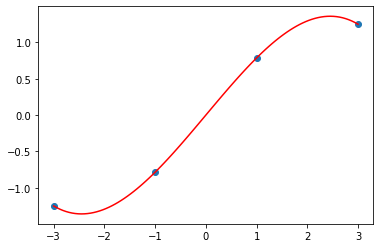
\includegraphics[scale=0.75]{3-1a}
\end{center}

Второй набор точек
\begin{center}
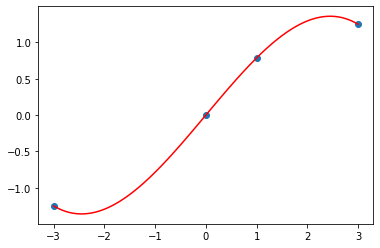
\includegraphics[scale=0.75]{3-1b}
\end{center}
\pagebreak

\subsubsection{Исходный код}
\lstinputlisting{../lab3_1/interpolator.hpp}
\pagebreak

\subsection{Сплай-интерполяция}

\subsubsection{Постановка задачи}
Построить кубический сплайн для функции, заданной в узлах интерполяции,
предполагая, что сплайн имеет нулевую кривизну при $x = x_0$ и $x = x_4$. Вычислить значение функции в точке $x = X^*$.

\subsubsection{Консоль}
\begin{alltt}
$ make
g++ -g -pedantic -std=c++17 -Wall -Wextra -Werror main.cpp -o solution
$ cat tests/2.in
5
-3.0 -1.0 1.0 3.0 5.0
-1.2490 -0.78540 0.78540 1.2490 1.3734
-0.5
$ ./solution < tests/2.in
Полученные сплайны:
i = 1, a = -1.2490, b = 0.0470, c = 0.0000, d = 0.0462
i = 2, a = -0.7854, b = 0.6014, c = 0.2772, d = -0.0926
i = 3, a = 0.7854, b = 0.5990, c = -0.2784, d = 0.0474
i = 4, a = 1.2490, b = 0.0542, c = 0.0060, d = -0.0010

Значение функции в точке x0 = -0.5000, f(x0) = -0.4270
\end{alltt}
\pagebreak

\subsubsection{Результат}
\begin{center}
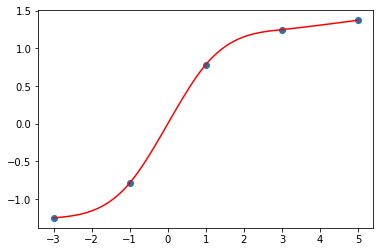
\includegraphics[scale=0.75]{3-2spline}
\end{center}
\pagebreak

\subsubsection{Исходный код}
\lstinputlisting{../lab3_2/cubic_spline.hpp}
\pagebreak

\subsection{Метод наименьших квадратов}

\subsubsection{Постановка задачи}
Для таблично заданной функции путем решения нормальной системы МНК найти приближающие многочлены a) 1-ой и б) 2-ой степени. Для каждого из приближающих многочленов вычислить сумму квадратов ошибок. Построить графики приближаемой функции и приближающих многочленов.

\subsubsection{Консоль}
\begin{alltt}
$ make
g++ -g -pedantic -std=c++17 -Wall -Wextra -Werror main.cpp -o solution
$ cat tests/2.in
6
-5.0 -3.0 -1.0 1.0 3.0 5.0
-1.3734 -1.249 -0.7854 0.7854 1.249 1.3734
$ ./solution < tests/2.in
Полученная функция первого порядка: 0.0000 0.3257
Значение суммы квадратов ошибков: 0.7007
Полученная функция второго порядка: 0.0000 0.3257 -0.0000
Значение суммы квадратов ошибков: 0.7007
\end{alltt}
\pagebreak

\subsubsection{Результат}
\begin{center}
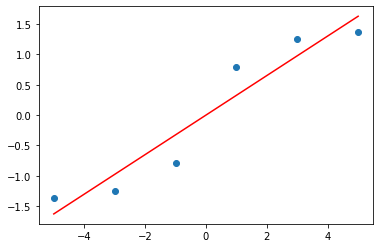
\includegraphics[scale=0.75]{3-3ms}
\end{center}
\pagebreak

\subsubsection{Исходный код}
\lstinputlisting{../lab3_3/minimal_square.hpp}
\pagebreak

\subsection{Численное дифференцирование}

\subsubsection{Постановка задачи}
Вычислить первую и вторую производную от таблично заданной функции $y_i = f(x_i)$, $i = 0, 1, 2, 3, 4$ в точке $x = X^*$.

\subsubsection{Консоль}
\begin{alltt}
$ make
g++ -g -pedantic -std=c++17 -Wall -Wextra -Werror main.cpp -o solution
$ cat tests/2.in
5
0.0 0.5 1.0 1.5 2.0
0.0 0.97943 1.8415 2.4975 2.9093
1.0
$ ./solution < tests/2.in
Первая производная функции в точке x0 = 1.0000, f'(x0) = 1.5181
Вторая производная функции в точке x0 = 1.0000, f''(x0) = -0.8243
\end{alltt}
\pagebreak

\subsubsection{Исходный код}
\lstinputlisting{../lab3_4/table_function.hpp}
\pagebreak

\subsection{Численное интегрирование}

\subsubsection{Постановка задачи}
Вычислить определенный интеграл $F = \int_{X_0}^{X_1}{y dx}$, методами прямоугольников, трапеций, Симпсона с шагами $h_1$, $h_2$. Оценить погрешность вычислений, используя Метод Рунге-Ромберга:

\subsubsection{Консоль}
\begin{alltt}
$ make
g++ -g -pedantic -std=c++17 -Wall -Wextra -Werror main.cpp -o solution
$ cat tests/1.in
0 2
0.5 0.25
$ ./solution < tests/1.in
Метод прямоугольников с шагом 0.5: 0.143739
Метод трапеций с шагом 0.5: 0.148748
Метод Симпсона с шагом 0.5: 0.145408

Метод прямоугольников с шагом 0.25: 0.144993
Метод трапеций с шагом 0.25: 0.146243
Метод Симпсона с шагом 0.25: 0.145409

Погрешность вычислений методом прямоугольников: 0.00167215
Погрешность вычислений методом трапеций: -0.0033396
Погрешность вычислений методом Симпсона: 1.56688e-06
\end{alltt}
\pagebreak

\subsubsection{Исходный код}
\lstinputlisting{../lab3_5/integrate.hpp}
\pagebreak
